\section{Fase I. Definición de requerimientos y restricciones}

    En esta fase se realizó una búsqueda en la literatura para establecer la estructura y dirección del proyecto, así como la incidencia del desarrollo tecnológico propuesto en determinados aspectos del mantenimiento, principalmente del sistema de información. Habiendo definido el mantenimiento preventivo en la sección \ref{subsec:preventive_maintenance}, se sabe que cuando una empresa trabaja en función de esta filosofía o metodología para controlar las actividades de manutención existe el manejo de cierta documentación técnica y logística, donde son de interés temas que rodean a la gestión de la información de mantenimiento, tanto en términos organizativos como en la sistematización del mismo.

    \subsection{Flujo de la información}

        En primera instancia uno de los aspectos que afectan al flujo de información es el cómo se concibe una empresa y en específico su sección de mantenimiento respecto a una estructura centralizada o descentralizada. La información manejada de forma centralizada tiene ventajas en su capacitación, manipulación y uso, además de disminuir las inconsistencias. Por su parte “la descentralización permite adaptar las necesidades del usuario, por lo tanto, motiva al usuario, facilita el reparto de las tareas y multiplica la eficacia de las funciones directivas” \parencite[p. 3]{ARRIBAS:2000}. Según \textcite[p. 7]{BEN-DAYA:2009} indica que en empresas de gran magnitud lo ideal es la estructura descentralizada, siendo la centralización lo recomendado para el caso de empresas de menor tamaño.

    \subsection{Tipos de información}

        Algunos ejemplos de que información debe ser registrada en el mantenimiento preventivo se encuentran listados en la Tabla \ref{tab:maintenance_data}. Complementario a esto, se presentan otras fuentes que respaldan y adicionan algunos puntos a considerar respecto al sistema de información de mantenimiento.

        Según la \textcite{COVENIN:1993} se describe a un sistema de información como “un conjunto de procedimientos interrelacionados, formales o informales, que permite la captura, procesamiento y flujo de información requerida en cada uno de los niveles de la organización” (p. 10), presentando procedimientos que contiene un sistema genérico de información de mantenimiento, donde se destacan:

        \begin{itemize}

            \item Inventario de los objetos del sistema productivo

            \item Codificación de los objetos de mantenimiento

            \item Registro de objetos de mantenimiento

            \item Instrucciones técnicas del mantenimiento

            \item Procedimiento de ejecución

            \item Programación del mantenimiento

            \item Historia de fallas de los equipos

        \end{itemize}

    \subsection{¿Donde incide el desarrollo tecnológico propuesto?}

        Según el \textcite[p. 6]{ICONTEC:2019} se dan pautas para desarrollar un sistema eficaz de gestión del conocimiento con el cual las empresas perciban una nueva fuente de generación de valor. Dentro de los puntos de la generación del conocimiento aparece la retención del conocimiento, lo cual se define como la capacidad de salvaguardar a la organización contra la pérdida de conocimiento. Asimismo se hacen anotaciones respecto a la protección del conocimiento en relación a las posibles rotaciones o variaciones del personal, además de tener la información documentada y respaldada.

        También se hace énfasis en la necesidad de incluir actividades y comportamientos para la transferencia de conocimientos listando cuatro ítems, siendo uno de ellos denominado la combinación donde se busca “sintetizar, conservar, formalizar, estructurar o clasificar el conocimiento codificado, haciendo que este sea accesible y fácil de encontrar” \parencite[p. 7]{ICONTEC:2019}. Con lo anterior se encuentran dos puntos de incidencia en el planteamiento del aplicativo de realidad aumentada y gestión de información de mantenimiento, en añadido al reconocimiento de las tecnologías como un apoyo a la gestión del conocimiento.

    \subsection{Análisis cualitativo} %%% podria ser una seccion

        Se optó por un enfoque cualitativo para llevar a cabo una investigación que resultara en la obtención de características y funcionalidades a incluir en un aplicativo que asista en la gestión de  información y desarrollo de actividades de mantenimiento. Este enfoque se caracteriza por su flexibilidad y la exploración de percepciones, acciones y sentimientos de participantes mediante entrevistas, análisis de contenido, observaciones o grupos focales \parencite{BARROGA:2023}.

    \subsection{Identificación de patrones}

        El análisis de los datos cualitativos implica procesos sistemáticos de codificación, categorización y síntesis de la información recopilada. Estos procesos no solo identifican patrones recurrentes, sino que también revelan las particularidades y variaciones que podrían no ser evidentes en los datos cuantitativos. Con lo anteriormente descrito en consideración, en esta fase metodológica se desarrolló una encuesta (Apéndice \ref{apc:qualitative_analysis_interview}) enfocada a adquirir datos y conceptos propuestos por los encuestados, que pudieran relacionarse entre sí y con base en ellos establecer características a incluir en un aplicativo móvil de realidad aumentada y de gestión de la información dirigido al campo del mantenimiento preventivo, así como para vislumbrar aspectos relacionados a este último.

        Se propusieron un total de catorce preguntas, donde se buscaban que los encuestados respondiesen en base a su experiencia en el área de mantenimiento, su cercanía tanto a las tecnologías de la información y la comunicación (TIC) así como a la realidad aumentada, problemáticas y conceptos relacionados al mantenimiento preventivo. Los perfiles de los encuestados corresponden a personal que a lo largo de su carrera se han involucrado en el campo de mantenimiento de equipos desde roles como ejecutor, educador, planificador o supervisor. Y además, las entrevistas fueron guardadas, registradas y anonimizadas para su respectivo análisis.

    \subsection{Codificación de las encuestas}

        En el análisis cualitativo, la codificación se refiere al proceso mediante el cual el investigador organiza progresivamente los datos en pequeños grupos o conjuntos con sentido, facilitando la comprensión de los fenómenos estudiados. Este procedimiento consiste en asignar etiquetas breves, ya sean palabras o frases concisas, a segmentos largos de texto, permitiendo representar y describir los procesos observados. Para ello, se debe construir una categorización de los códigos, la cual, según \textcite{RODRIGUEZ:2005}, puede estructurarse a partir de uno de los siguientes enfoques metodológicos:

        \begin{quote}
        
            El primero es el llamado inductivo y consiste en elaborar las categorías a partir de la lectura y examen del material recopilado sin tomar en consideración categorías de partida (...). El segundo es el denominado deductivo, en el que, al contrario del anterior, las categorías están establecidas a priori, siendo función del investigador adaptar cada unidad a una categoría ya existente. Por último, se encuentra el proceso mixto, a través del cual el investigador tomaría como categorías de partida las existentes, formulando alguna más cuando este repertorio de partida se muestre ineficaz, es decir, que no contenga dentro de su sistema de categorías ninguna capaz de cubrir alguna unidad de registro (p. 141).

        \end{quote}

        \subsubsection{Categorización}

            Para lograr enlazar o relacionar lo expresado en las entrevistas se enumeraron categorías, sub-categorías y palabras clave, las cuales identifican una determinada frase de interés dentro del cuerpo de texto de las transcripciones, y así poder ligar diferentes citas de los entrevistados a un tema específico, encontrando similitudes o repeticiones en algunos términos. Las categorías generadas fueron las siguientes:

            \begin{itemize}

                \item \textbf{Perfil del encuestado:} donde se clasificó la información en base a la experiencia de los encuestados en el mantenimiento, los conocimientos asociados a dicha experiencia y la cercanía que tienen con el uso de tecnologías en este mismo contexto.

                \item \textbf{Mantenimiento preventivo:} donde se clasificó aquella información relacionada con aspectos y conocimientos de mantenimiento.

                \item \textbf{Defectos organizacionales:} donde se describen principalmente problemáticas que pueden presentarse en un contexto de mantenimiento de equipos, cuyo impacto negativo puede ser disminuido con la inclusión de nuevas tecnologías como la que se propone en el presente proyecto.

                \item \textbf{Aplicativo de realidad aumentada:} donde se clasificó información asociada con características y funcionalidades de un aplicativo de realidad aumentada para mantenimiento preventivo, así como los desafíos de su implementación.

            \end{itemize}

            \begin{figure}[H]

    \caption{Categorización de los códigos para análisis cualitativo.}
    
    \centering
    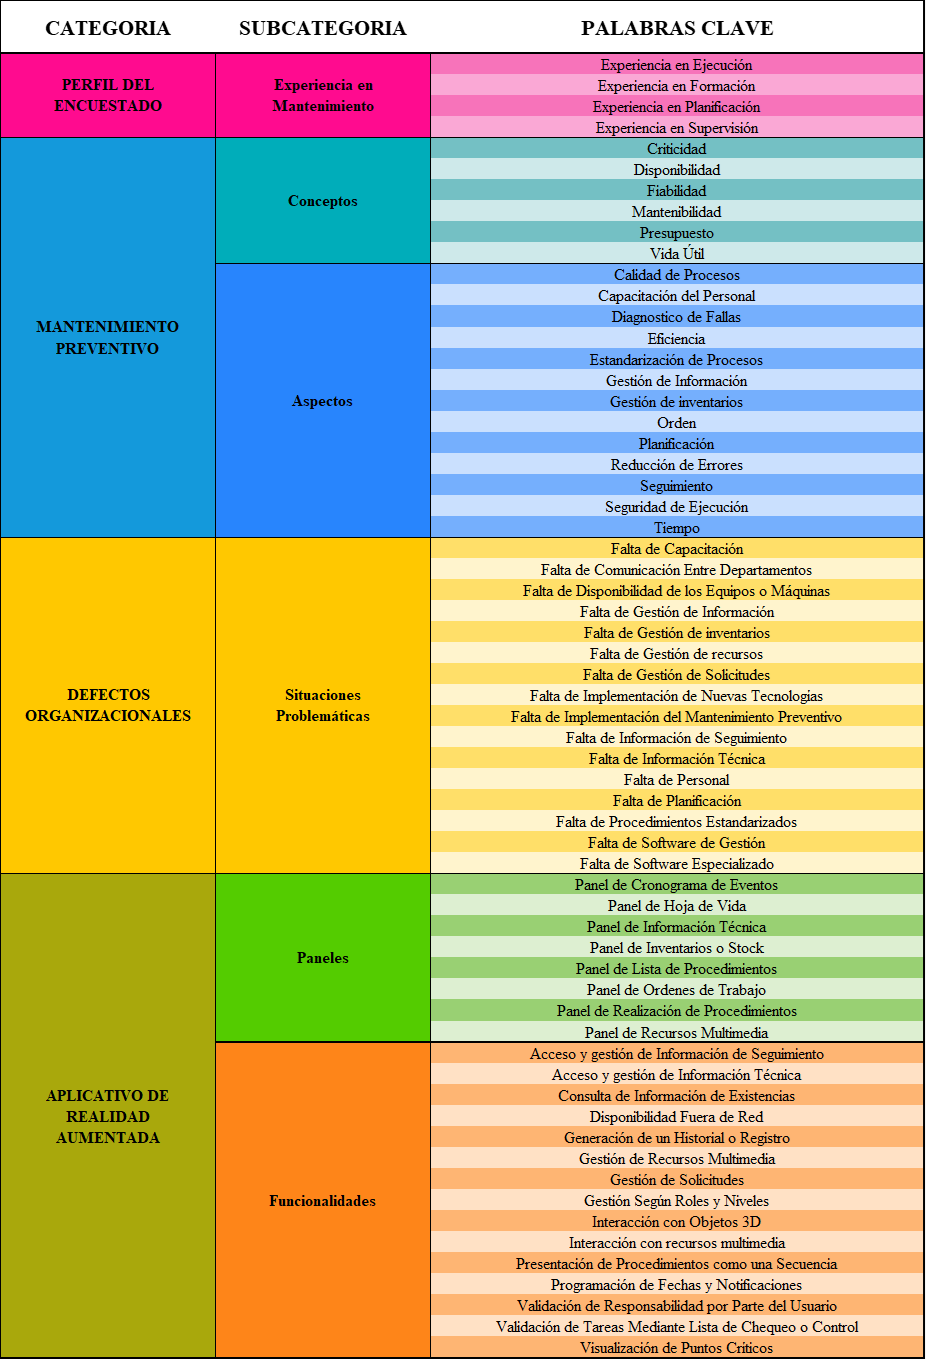
\includegraphics[width=0.9\textwidth]{assets/images/codes_categories.png}
    \label{fig:codes_categories}
    
\end{figure}
\vspace{-1.6\baselineskip}

            En la Figura \ref{fig:codes_categories} se presentan las palabras clave y las subcategorías que fueron utilizadas como códigos en el software de análisis cualitativo ATLAS.ti. Varias de estas palabras clave corresponden a lo que se denomina un “código emergente”, característico del enfoque inductivo, especialmente aquellas relacionadas con funcionalidades y características.

    \subsection{Uso de software de análisis cualitativo}

        Con los documentos de las transcripciones cargados en el área de trabajo de ATLAS.ti, se llevó a cabo una lectura con el objetivo de seleccionar citas de interés y asignar los códigos que tenían relación con las mismas. Se resalta que una cita puede hablar de diferentes palabras clave, lo cual resulta en que estará ligada a distintos códigos; con lo anterior se generan relaciones tanto de densidad, co-ocurrencia y semántica entre los códigos pudiendo identificar con estas la relevancia que las personas encuestadas daban a un término en específico.

        %%%%%%%%%% MOVER AQUI LOS SANKEY

    \subsection{Creación de redes semánticas}

        Siguiendo la línea del análisis cualitativo y con el objetivo de identificar relaciones entre los conceptos e ideas emergentes durante la categorización y codificación, se recurre al uso de redes semánticas, también conocidas como redes conceptuales. Estas estructuras presentan un patrón característico que les permite vincular diversos nodos y representar cómo se interrelacionan dos palabras o conceptos \parencite{PEREZ:2022}.  %%%% revisar "y" griega y tal vez num. pag.

        Se generaron redes semánticas para cada uno de los paneles identificados en las encuestas, con el fin de explorar qué funcionalidades deberían incluirse y qué aspectos del mantenimiento se relacionan con cada uno. Estas redes permiten visualizar posibles enfoques para el diseño del aplicativo de realidad aumentada, brindando un conjunto de opciones que orientan la toma de decisiones en función de cuáles se alinean mejor con los objetivos del sistema. El software utilizado ofrece siete tipos de relaciones conceptuales por defecto (Figura \ref{fig:default_relations_atlasti}), aunque se propusieron nuevos conectores personalizados (Figura \ref{fig:proposed_relation_connectors}) para representar con mayor precisión las relaciones entre códigos.

        \begin{figure}[H]%htbp

    \caption{Relaciones por defecto de ATLAS.ti.}
    
    \centering
    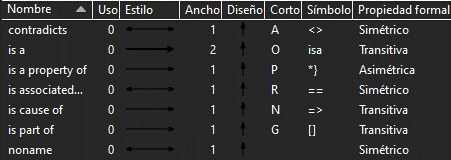
\includegraphics[width=0.6\textwidth]{assets/images/default_relations_atlasti.png}
    \label{fig:default_relations_atlasti}
    
\end{figure}
\vspace{-0.8\baselineskip}

        \begin{figure}[H]

    \caption{Conectores de relación propuestos.}
    
    \centering
    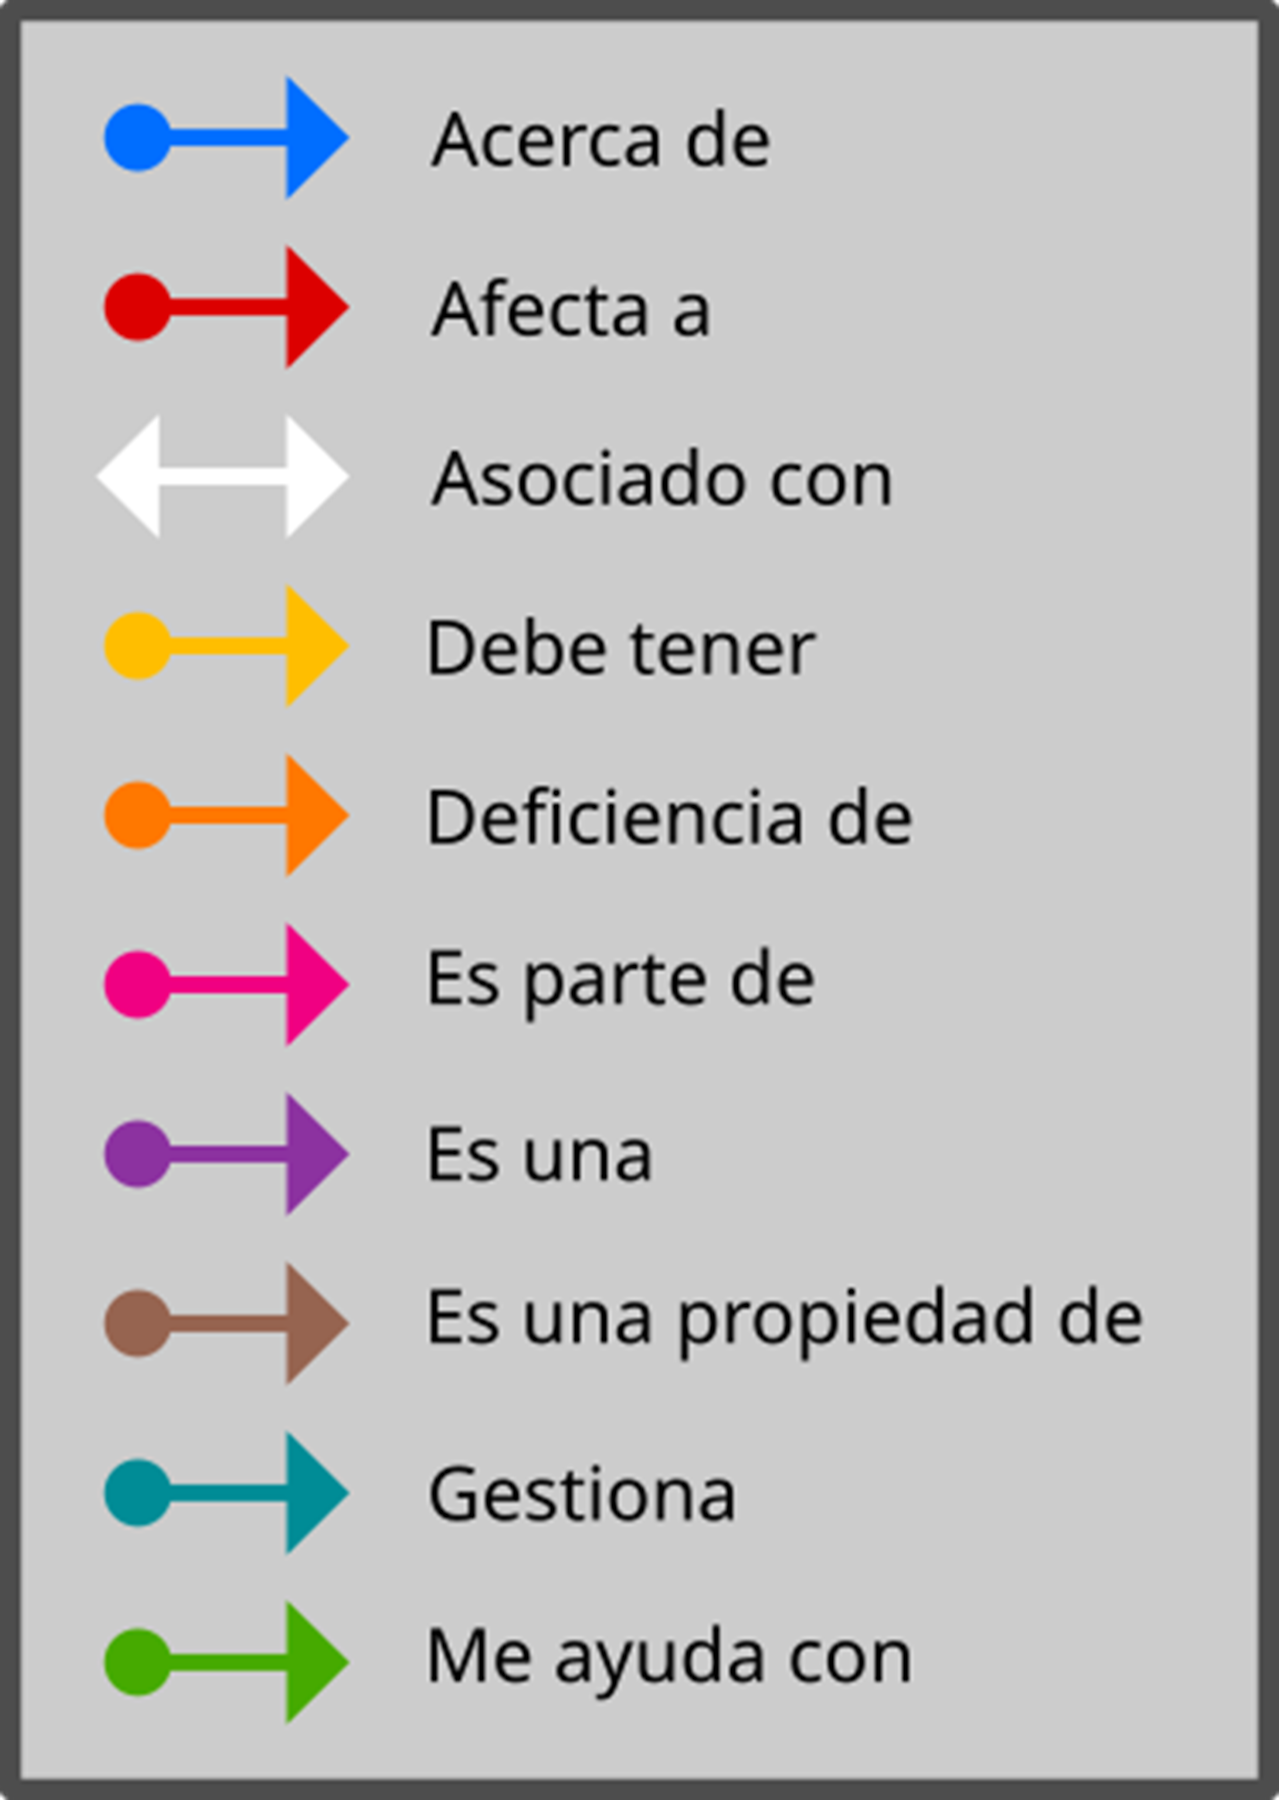
\includegraphics[width=0.3\textwidth]{assets/images/proposed_relation_connectors.png}
    \label{fig:proposed_relation_connectors}
    
\end{figure}
\vspace{-0.8\baselineskip}

        \subsubsection{Redes semánticas de los paneles}

            Las redes desarrolladas, correspondientes a los paneles identificados durante la codificación, se conectan principalmente con funcionalidades del aplicativo. A su vez, estas funcionalidades se relacionan con aspectos y conceptos del mantenimiento, ya que su implementación busca mejorar directamente dichos elementos.
            
            \paragraph{Panel de cronograma de eventos} mostrado en la Figura \ref{fig:semantic_network_schedule}, tiene implicaciones en la gestión de la información relacionada con el tiempo, siendo la planificación una propiedad asociada al mismo. Este panel permite la programación y notificación de fechas, donde la gestión de los tiempos de intervención se asocian directamente con el concepto de vida útil.

            \begin{figure}[H]

    \caption{Relaciones semánticas del panel de cronograma}
    
    \centering
    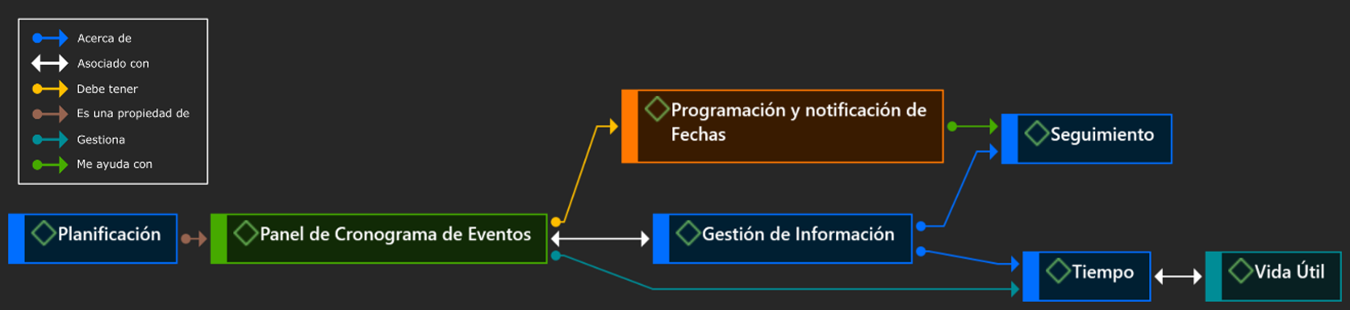
\includegraphics[width=1.0\textwidth]{assets/images/semantic_network_schedule.png}
    \label{fig:semantic_network_schedule}
    
\end{figure}
\vspace{-1.6\baselineskip}

            \paragraph{Panel de recursos multimedia} mostrado en la Figura \ref{fig:semantic_network_media_resources}, se enfoca en la gestión de manuales, fichas técnicas y otros documentos relacionados con los equipos y procesos de mantenimiento. Este panel permite al usuario acceder e interactuar con dicha información desde el aplicativo, facilitando también la capacitación y familiarización con los equipos.

            \begin{figure}[H]%htbp

    \caption{Relaciones semánticas del panel de recursos multimedia}
    
    \centering
    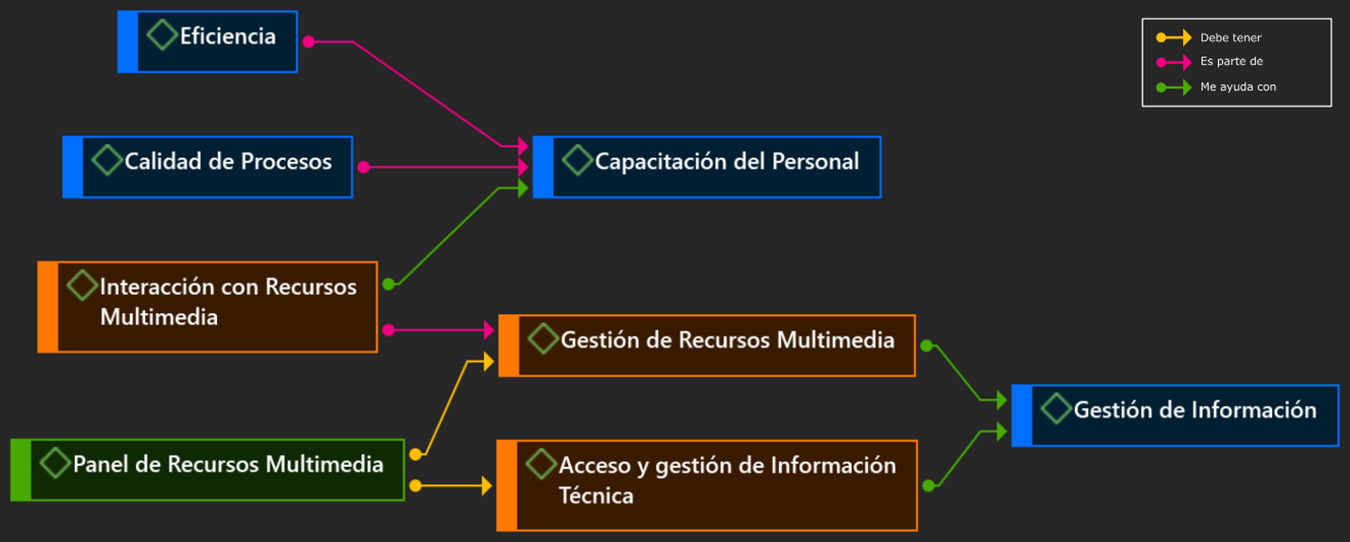
\includegraphics[width=1.0\textwidth]{assets/images/semantic_network_media_resources.png}
    \label{fig:semantic_network_media_resources}
    
\end{figure}
\vspace{-1.6\baselineskip}

            \paragraph{Panel de inventario} mostrado en la Figura \ref{fig:semantic_network_inventory}, permite consultar la información de existencias para evitar errores en el conteo de disponibilidad antes y después de las intervenciones. Además, facilita el acceso a las características y especificaciones técnicas de los elementos registrados en el inventario.

            \begin{figure}[H]%htbp

    \caption{Relaciones semánticas del panel de inventario}
    
    \centering
    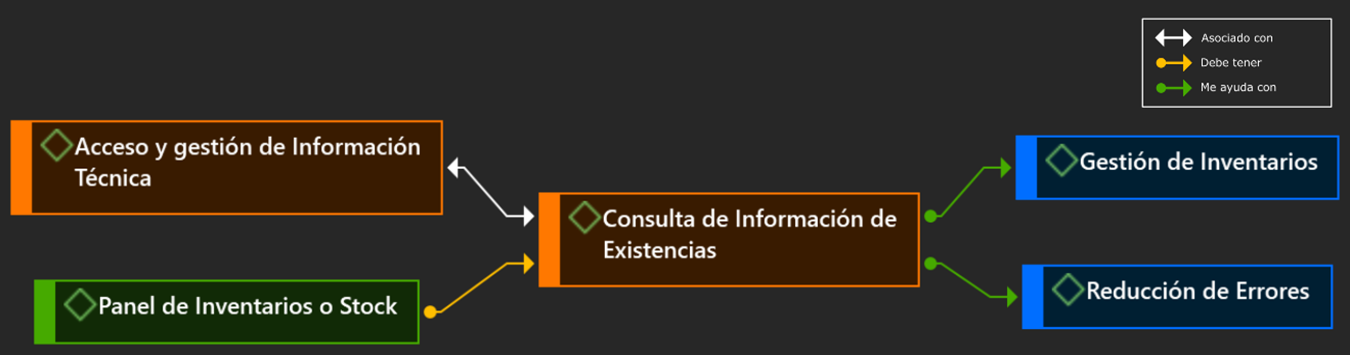
\includegraphics[width=1.0\textwidth]{assets/images/semantic_network_inventory.png}
    \label{fig:semantic_network_inventory}
    
\end{figure}
\vspace{-1.6\baselineskip}

            \paragraph{Panel de realización de procedimientos} mostrado en la Figura \ref{fig:semantic_network_procedures_development}, destaca la interacción con objetos 3D durante la ejecución de tareas. Esta característica propia de la realidad aumentada funciona como guía visual para el usuario encargado del mantenimiento, facilitando el aprendizaje y la correcta ejecución de los procedimientos.

            \begin{figure}[H]%htbp

    \caption{Relaciones semánticas del panel de realización de procedimientos}
    
    \centering
    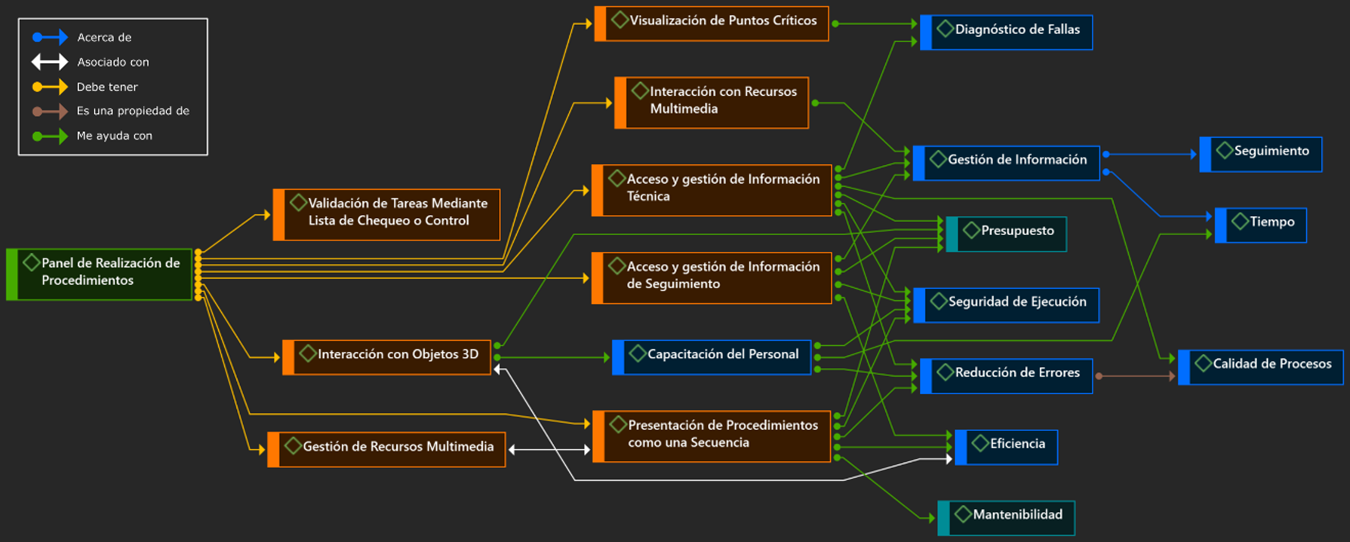
\includegraphics[width=1.0\textwidth]{assets/images/semantic_network_procedures_development.png}
    \label{fig:semantic_network_procedures_development}
    
\end{figure}
\vspace{-1.6\baselineskip}

            \paragraph{Panel de lista de procedimientos} mostrado en la Figura \ref{fig:semantic_network_procedures_list}, presenta los procedimientos organizados como una secuencia estructurada. Esta forma de visualización permite al usuario seguir paso a paso las instrucciones necesarias, apoyando la comprensión y cumplimiento adecuado de cada tarea.

            \begin{figure}[H]%htbp

    \caption{Relaciones semánticas del panel de lista de procedimientos}
    
    \centering
    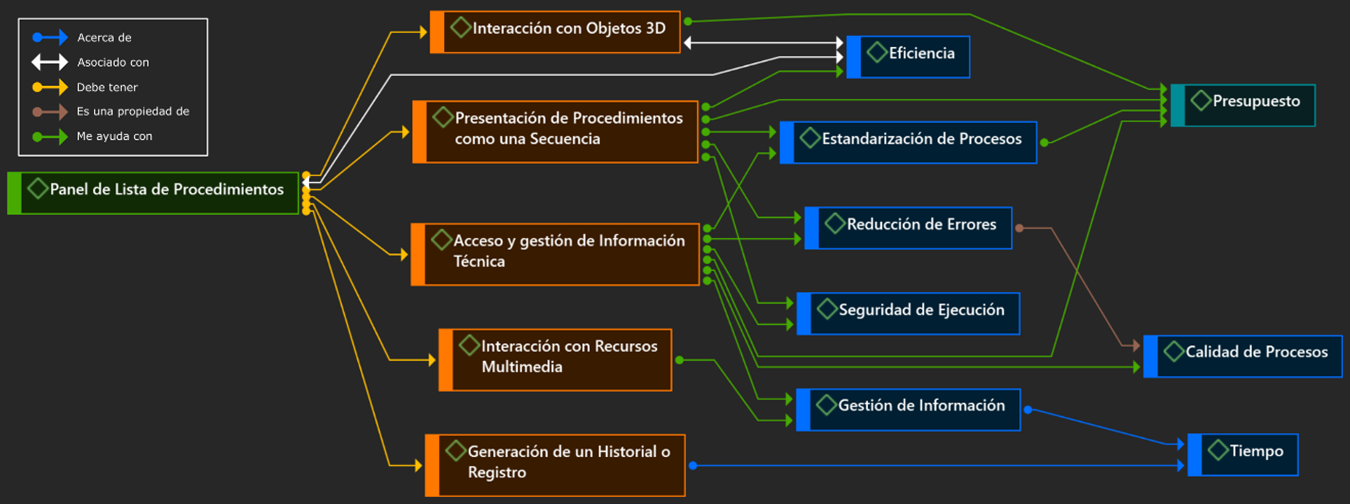
\includegraphics[width=1.0\textwidth]{assets/images/semantic_network_procedures_list.png}
    \label{fig:semantic_network_procedures_list}
    
\end{figure}
\vspace{-1.6\baselineskip}

            \paragraph{Panel de información técnica} mostrado en la Figura \ref{fig:semantic_network_technical_information}, agrupa funcionalidades relacionadas con la interacción con recursos multimedia y la gestión de información técnica y de seguimiento. Se destacó además la necesidad de disponibilidad fuera de red, especialmente para acceder a documentación y recursos sin conexión a internet.

            \begin{figure}[H]

    \caption{Relaciones semánticas del panel de información técnica}

    \centering
    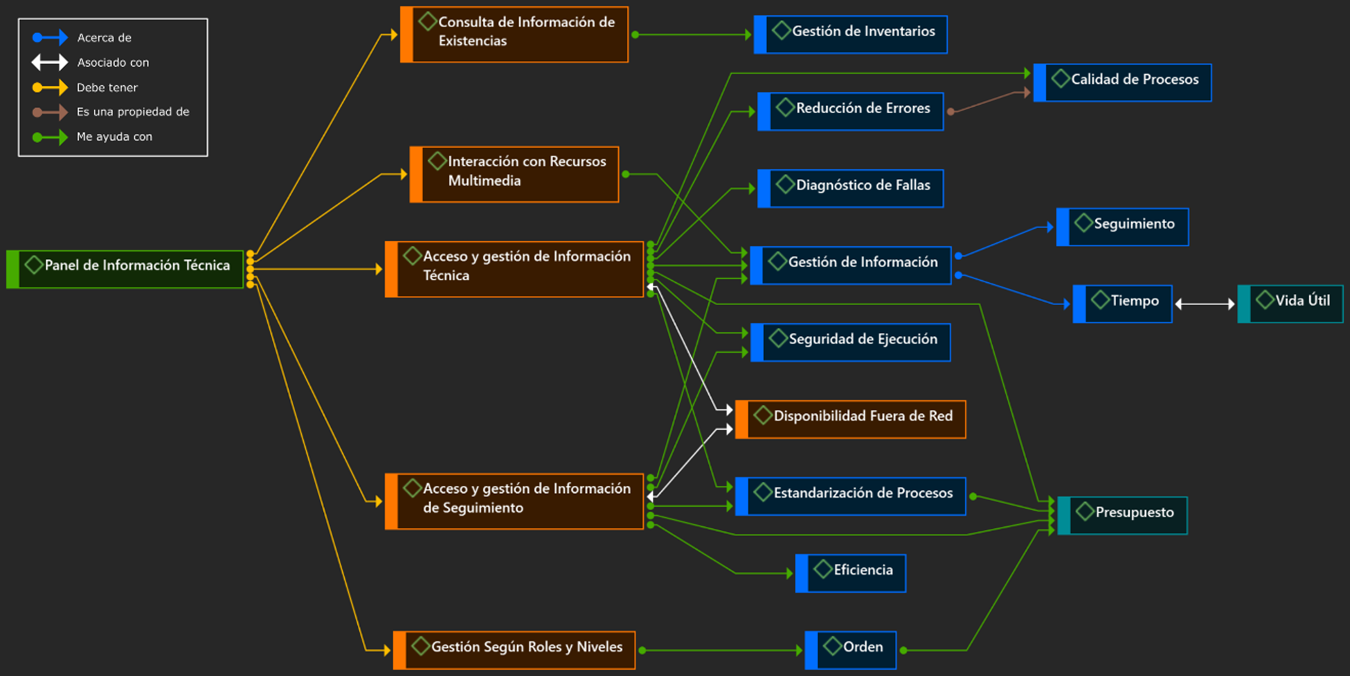
\includegraphics[width=1.0\textwidth]{assets/images/semantic_network_technical_information.png}
    \label{fig:semantic_network_technical_information}
    
\end{figure}
\vspace{-1.6\baselineskip}

            \paragraph{Situaciones problemáticas en el mantenimiento} presenta una red semántica a partir de las situaciones problemáticas reportadas por los entrevistados. Estas situaciones, basadas en su experiencia en tareas de mantenimiento en distintas instituciones, se relacionan principalmente con algunos aspectos de mantenimiento, identificados tanto como causas o como consecuencias.

            \begin{figure}[H]%htbp

    \caption{Relaciones semánticas de las situaciones problemáticas}
    
    \centering
    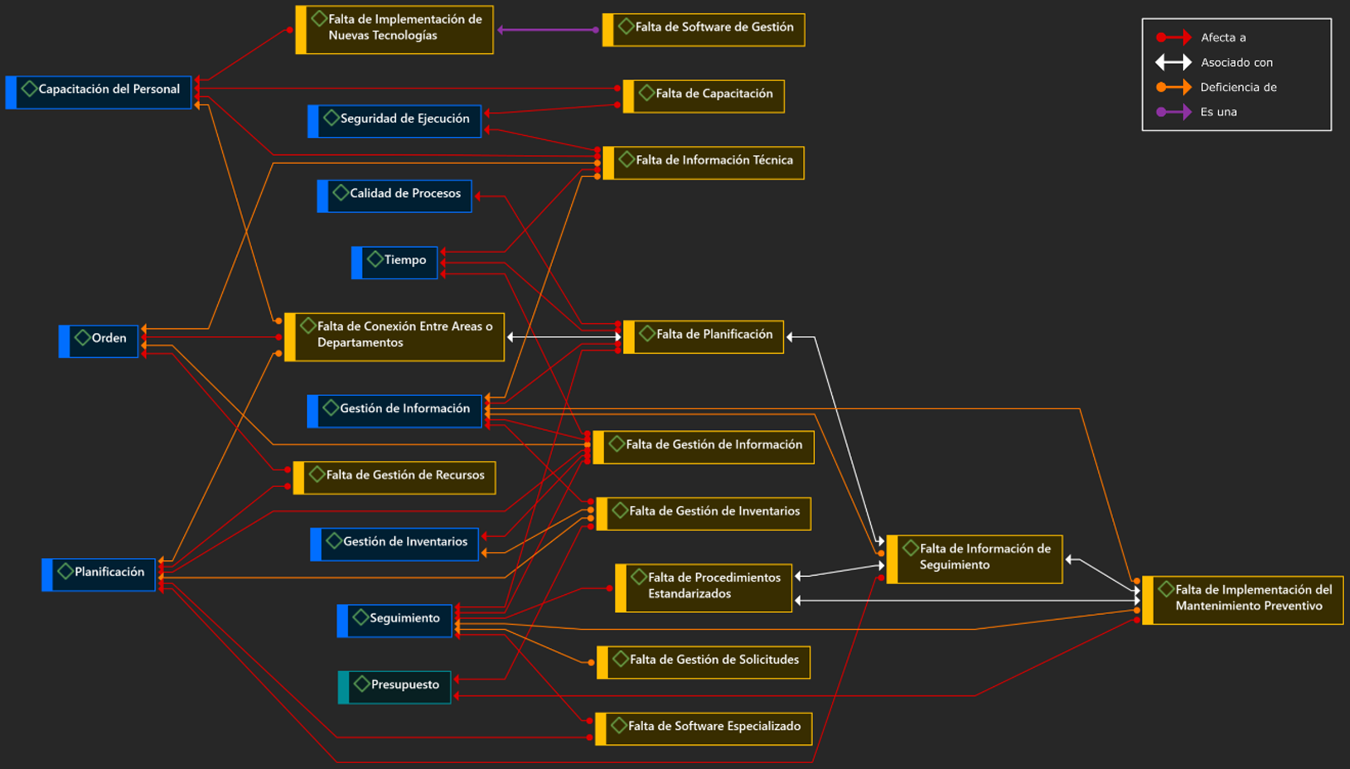
\includegraphics[width=1.0\textwidth]{assets/images/semantic_network_problematic_situations.png}
    \label{fig:semantic_network_problematic_situations}
    
\end{figure}
\vspace{-1.6\baselineskip}

    \subsection{Co-ocurrencia de datos}

        Uno de los elementos o aspectos a visualizar fue la  co-ocurrencia, "la cual se refiere a los casos en que dos o más códigos aparecen juntos en el mismo contexto de datos (…). La co-ocurrencia puede revelar temas o patrones en los datos, ayudando a los investigadores a comprender las complejas relaciones entre los distintos elementos de su estudio" \parencite{STEWART:SF}.

        \subsubsection{Diagramas Sankey}

            La aparición de relaciones entre códigos intuyen una conexión donde se optó el uso de diagramas Sankey, los cuales permiten visualizar la proporción de un código o concepto en relación con otros.

            \paragraph{Diagrama de densidad de las funcionalidades}representado en la Figura \ref{fig:sankey_functionalities}, muestra la relevancia que los encuestados dieron a cuales podrían ser las prestaciones incluidas dentro de los distintos paneles o secciones gráficas del aplicativo, donde se destacaron el acceso y gestión de la información técnica, además de poder interactuar con objetos 3D con procedimientos secuenciales, acercándose a la propuesta de hacer uso de la realidad aumentada para las intervenciones de mantenimiento.

            \begin{figure}[H]%htbp

    \caption{Densidad de las funcionalidades del aplicativo resaltadas por los encuestados}
    
    \centering
    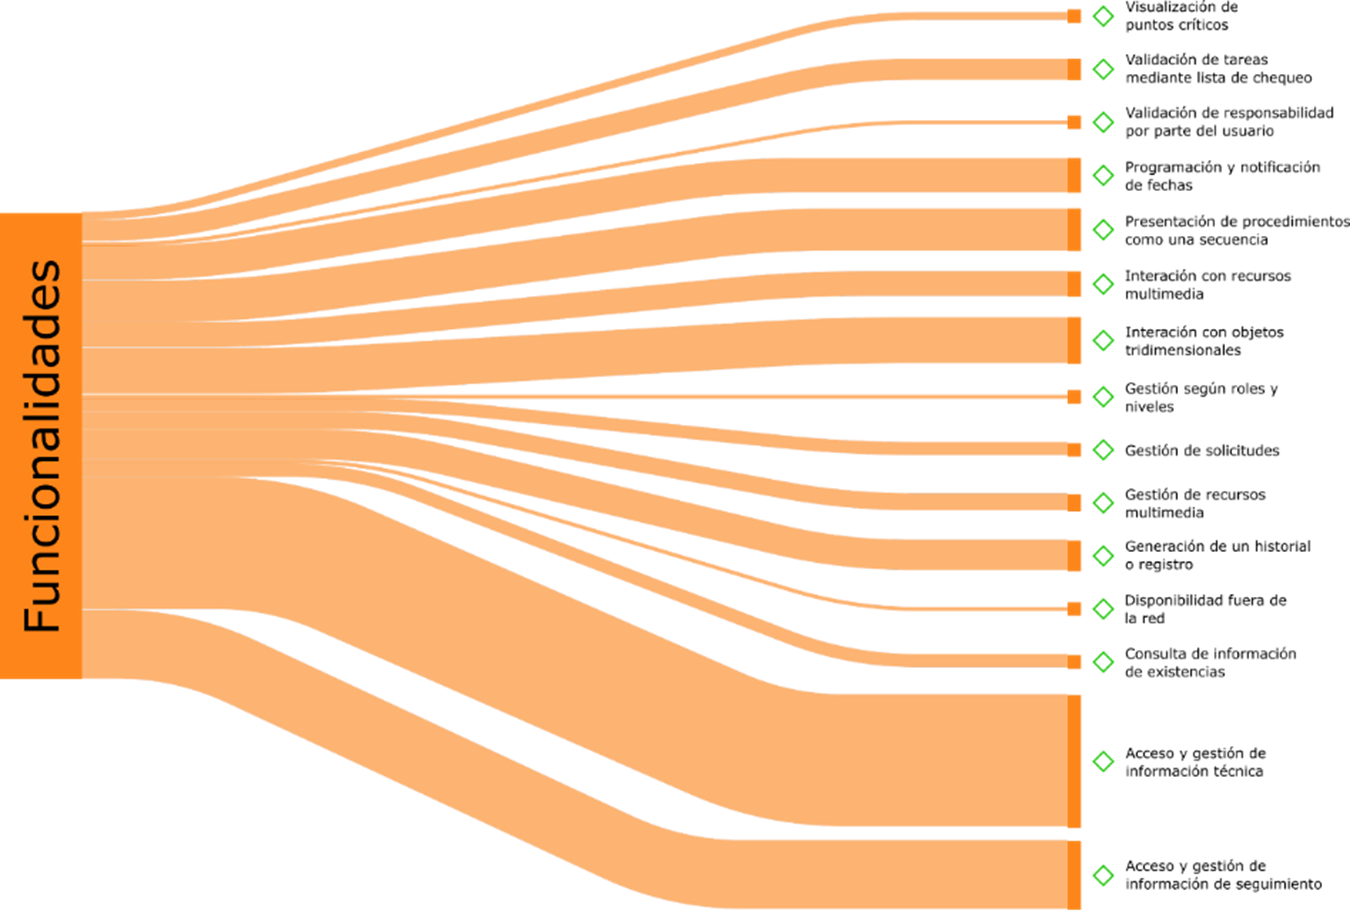
\includegraphics[width=0.8\textwidth]{assets/images/sankey_functionalities.png}
    \label{fig:sankey_functionalities}
    
\end{figure}
\vspace{-0.8\baselineskip}

            \paragraph{Diagrama de densidad de experiencia en mantenimiento} representado en la Figura \ref{fig:sankey_maintenance_experience} muestra la proporción en la experiencia que han tenido los encuestados donde se observa que la mayor densidad está hacia la parte de ejecución de mantenimiento.

            \begin{figure}[H]%htbp

    \caption{Densidad de la experiencia en mantenimiento de los encuestados}
    
    \centering
    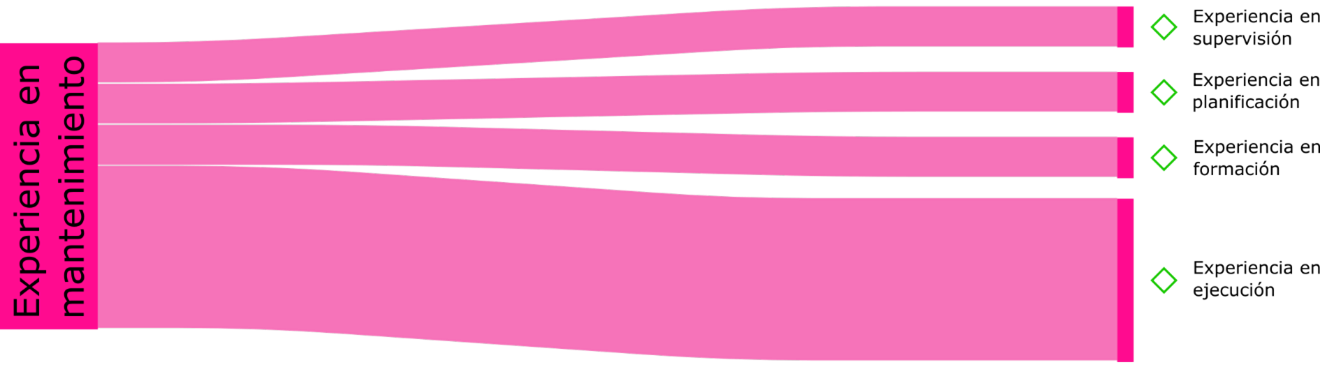
\includegraphics[width=0.8\textwidth]{assets/images/sankey_maintenance_experience.png}
    \label{fig:sankey_maintenance_experience}
    
\end{figure}
\vspace{-0.8\baselineskip}

            \paragraph{Diagrama de densidad de los paneles} representado en la Figura \ref{fig:sankey_panels} identifica las propuestas de las secciones gráficas que pueden ser incluidas en el aplicativo, donde se observa una alta mención al panel de información técnica prevaleciendo la importancia de los aspectos de gestión de información técnica específica de los ítems mantenibles y del mismo modo se observa una gran densidad al panel de realización de procedimientos y el de lista de procedimientos, siendo estos una guía en el desarrollo de las distintas intervenciones de mantenimiento con el uso de realidad aumentada.

            \begin{figure}[H]%htbp

    \caption{Densidad de los paneles del aplicativo de mantenimiento}
    
    \centering
    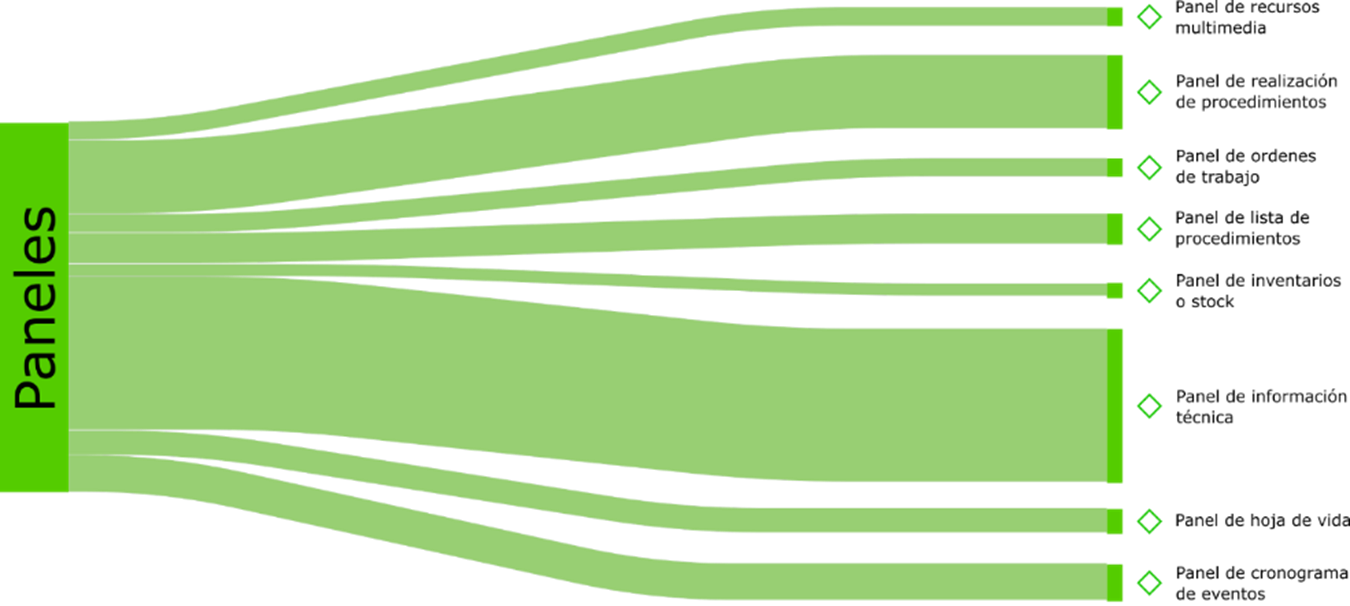
\includegraphics[width=0.8\textwidth]{assets/images/sankey_panels.png}
    \label{fig:sankey_panels}
    
\end{figure}
\vspace{-0.8\baselineskip}
            
            \paragraph{Diagrama de co-ocurrencia entre funcionalidades y aspectos de mantenimiento} representado en la Figura \ref{fig:sankey_coocurrence_functionalities_aspecs}, se  observar un patrón de divergencia en el que ciertas funcionalidades (representadas de color naranja) se conectan con múltiples aspectos de mantenimiento (representados de color azul), el cual puede indicar un carácter multifacetico dentro del aplicativo de realidad aumentada. A su vez se observa un patron de convergencia donde multiples funcionalidades se relacionan con un mismo aspecto de mantenimiento las cuales podrían indicar criterios clave de diseño o experiencia de usuario, ya que son considerados desde distintas funcionalidades.
            
            \input{assets/figures/sankey_coocurrence_functionalities_aspecs.tex}

            \paragraph{Diagrama de co-ocurrencia entre funcionalidades y conceptos de mantenimiento} representado en la Figura \ref{fig:sankey_coocurrence_functionalities_concepts} se observan del mismo modo patrones de divergencia donde ciertas funcionalidades (representadas de color naranja) se conectan con multiples conceptos clave de mantenimiento (representados de color celeste) indicando una conexión teórica, la cual ayuda a identificar cuales funcionalidades pueden ser mejor acopladas a características propias de un sistema de realidad aumentada.

            \input{assets/figures/sankey_coocurrence_functionalities_concepts.tex}

            \paragraph{Diagrama de co-ocurrencia entre paneles y funcionalidades} representado en la Figura \ref{fig:sankey_coocurrence_panels_functionalities} muestra una divergencia entre ciertos paneles (representados de color verde) conectados a multiples funcionalidades (representados de color naranja), indicando una sección del aplicativo sea de carácter central o multifuncional, donde se puede guiar al usuario a través de la presencia o accesibilidad a ciertas funciones, permitiendo la identificación funcionalidades principales y facilitando la organización y desarrollo de la aplicación de realidad aumentada. 

            \begin{figure}[H]

    \caption{Co-ocurrencia entre los paneles propuestos y funcionalidades de mantenimiento}
    
    \centering
    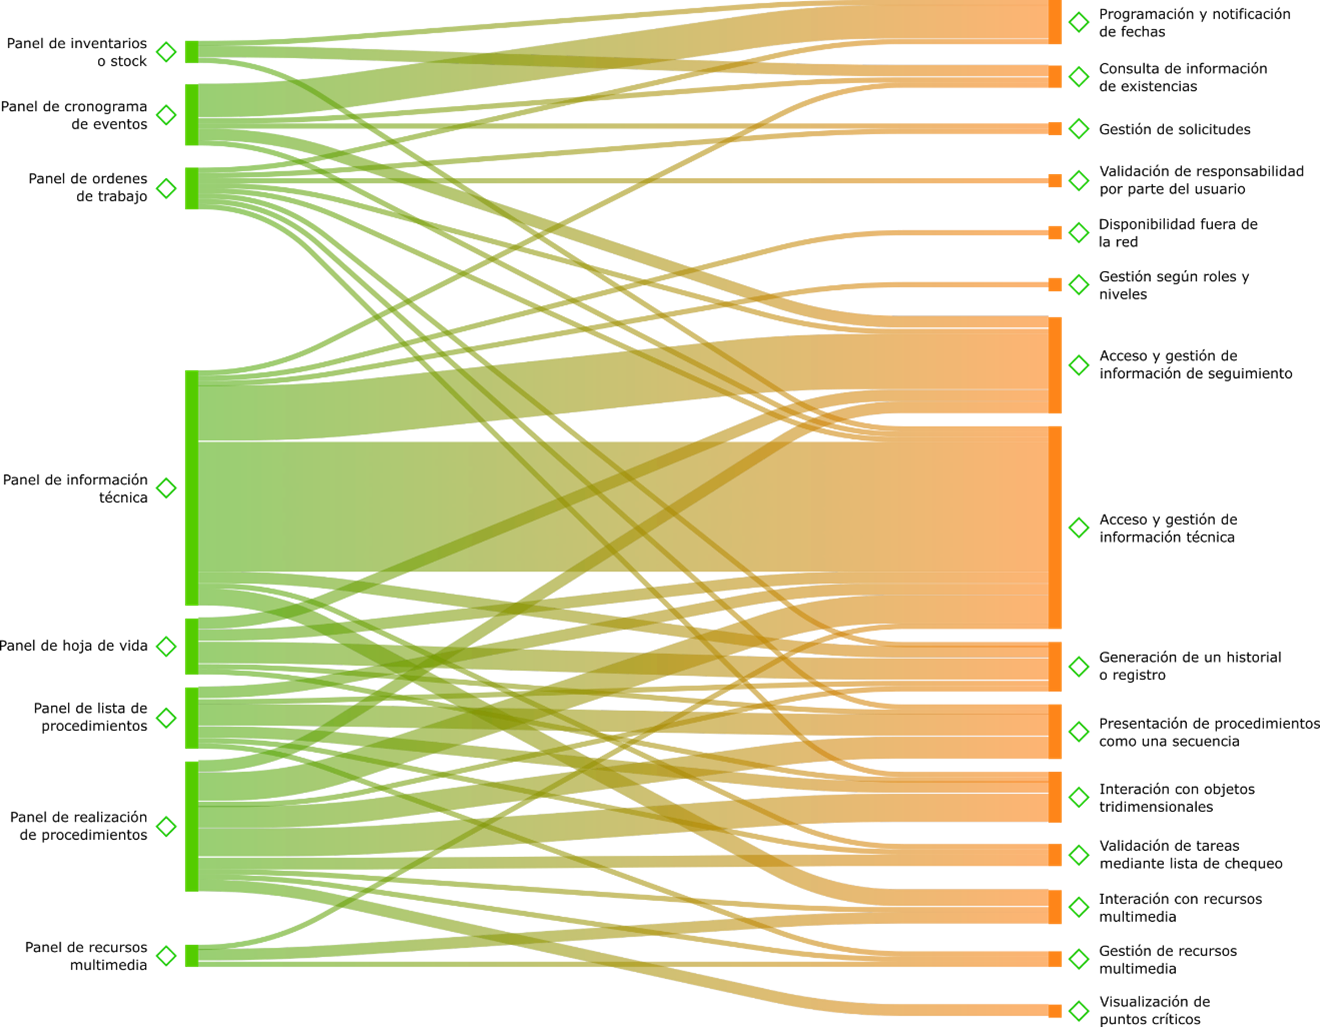
\includegraphics[width=1.0\textwidth]{assets/images/sankey_coocurrence_panels_functionalities.png}
    \label{fig:sankey_coocurrence_panels_functionalities}
    
\end{figure}
\vspace{-1.6\baselineskip}